\section{Capturas de Gameplay}

As capturas apresentadas nesta seção foram obtidas pelo próprio grupo
durante sessões de gameplay dos jogos analisados. Elas são utilizadas
como evidência visual complementar para a análise dos elementos gráficos,
texturas, materiais e superfícies apresentados nos jogos.

\section{Rocket League}

As Figuras abaixo apresentam capturas próprias realizadas durante o
gameplay de \textit{Rocket League}. As imagens permitem observar
diferentes elementos visuais do jogo, incluindo veículos, superfícies
e elementos do ambiente.

\begin{figure}[H]
    \centering
    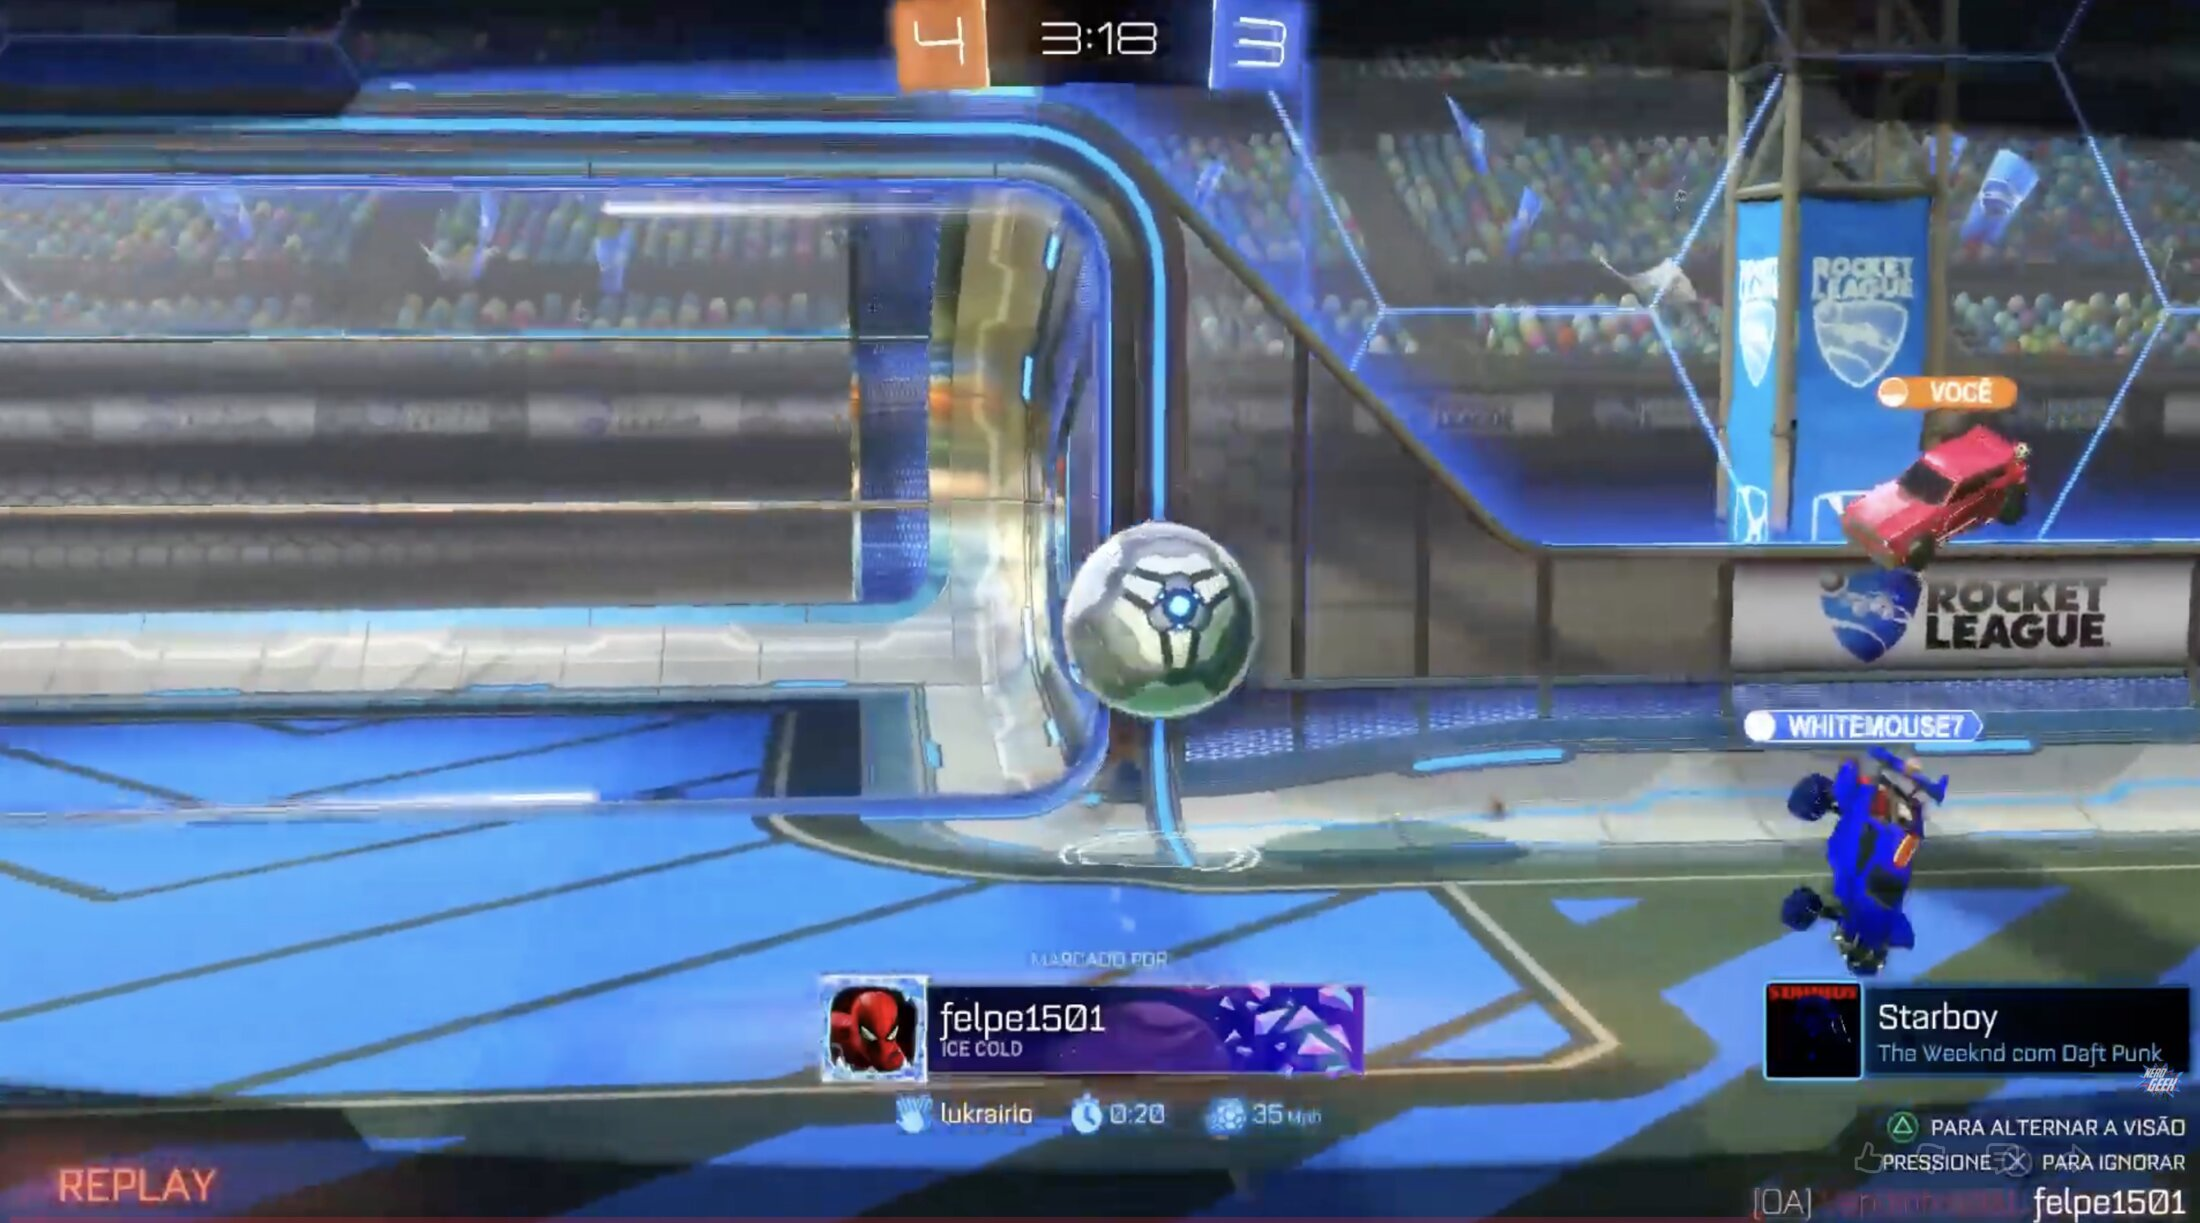
\includegraphics[width=0.9\textwidth]{imagens/rocket_league/rocket_league.jpg}
    \caption{Captura própria de \textit{Rocket League} durante o gameplay.}
    \label{fig:rocket-league}
\end{figure}

\begin{figure}[H]
    \centering
    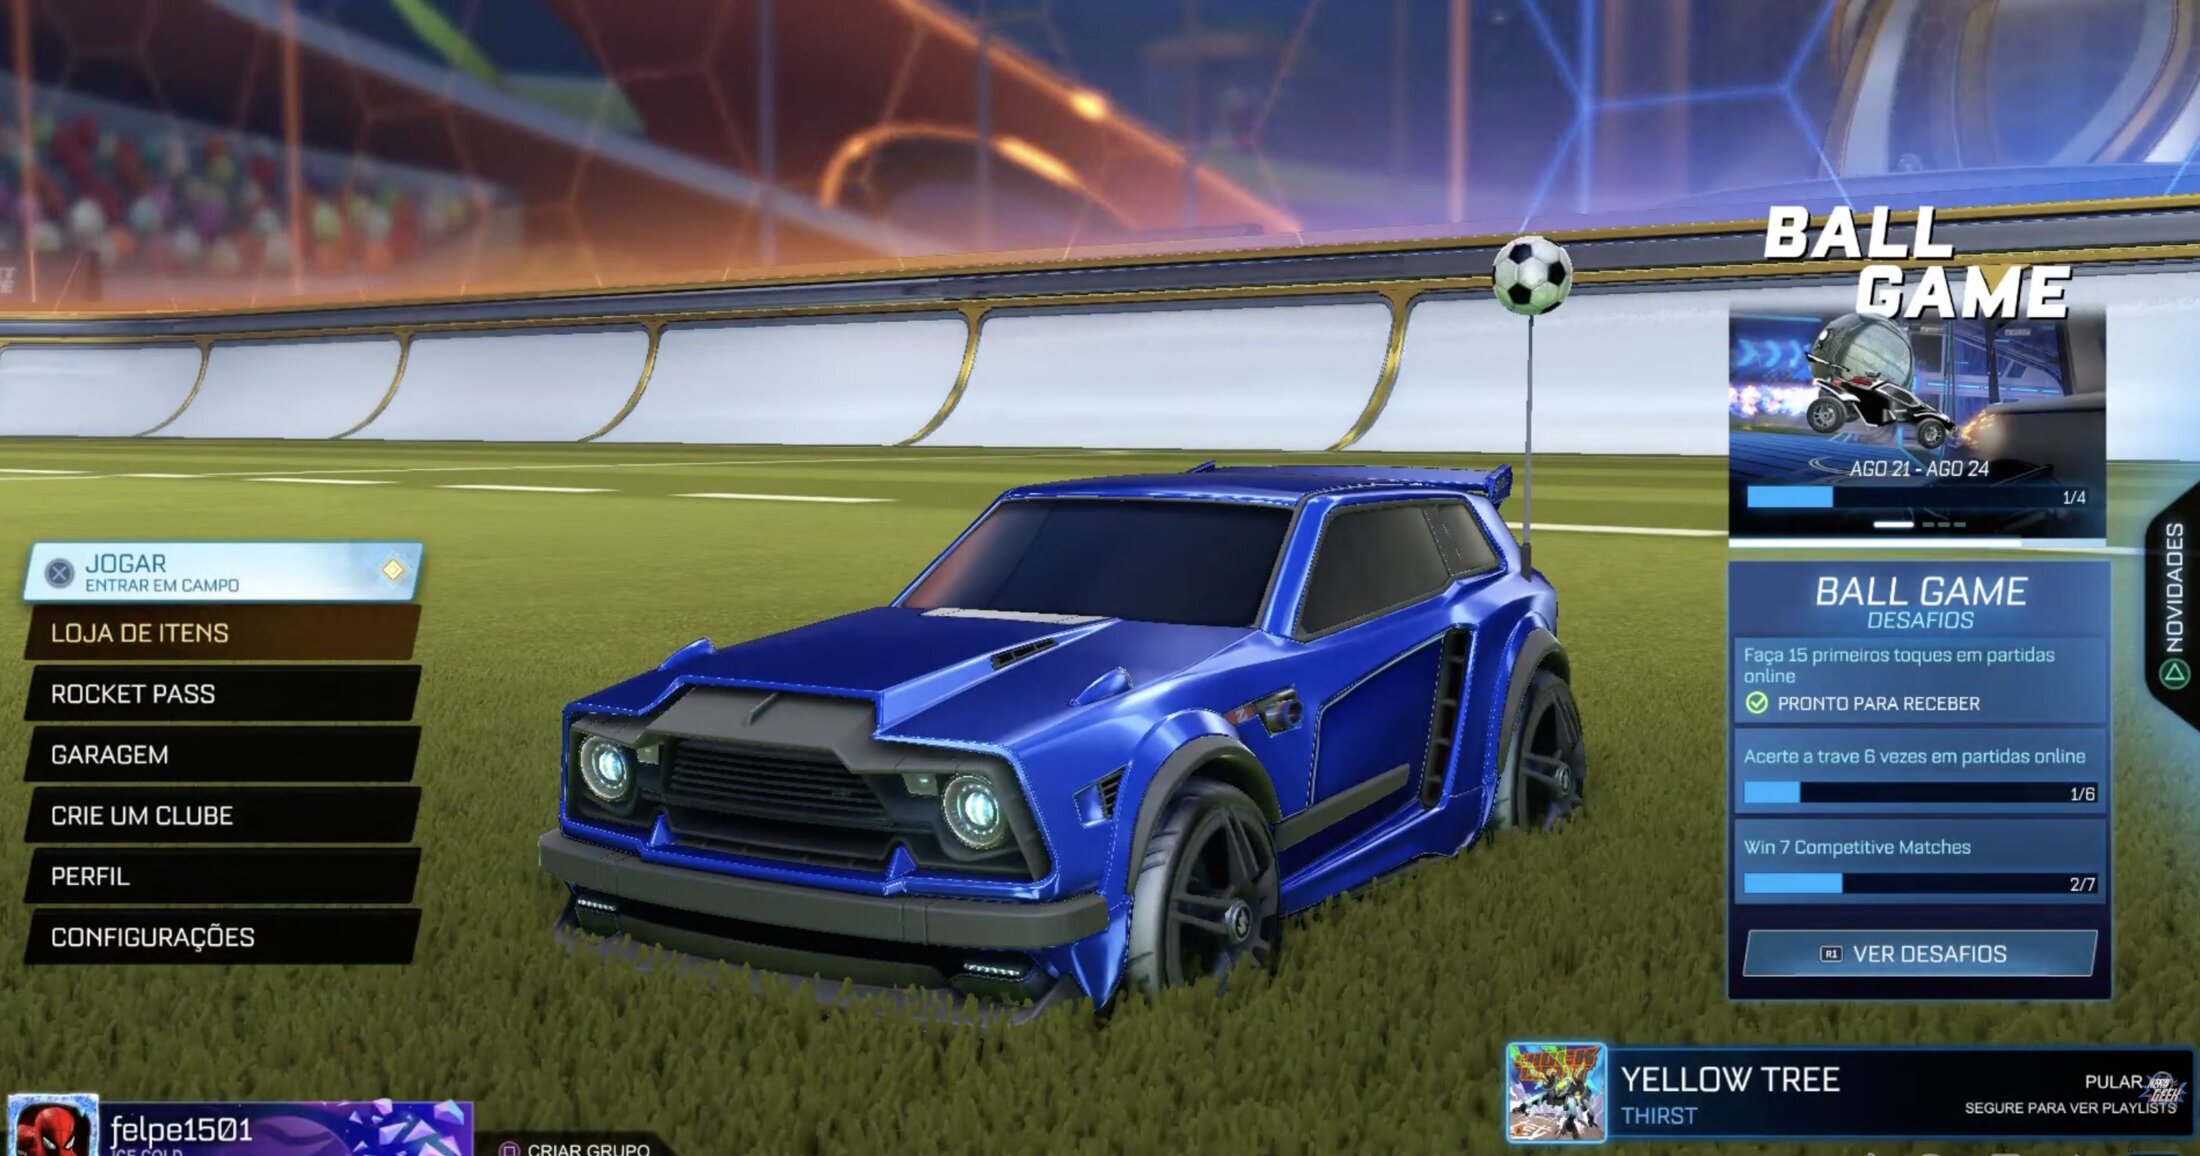
\includegraphics[width=0.9\textwidth]{imagens/rocket_league/rocket_league01.jpg}
    \caption{Segunda captura própria de \textit{Rocket League}.}
    \label{fig:rocket-league-01}
\end{figure}

As capturas complementam a análise apresentada na seção de jogos,
permitindo visualizar diretamente os elementos gráficos presentes
durante a execução do jogo.

\section{Marvel's Spider-Man Remastered}

As Figuras abaixo apresentam capturas próprias realizadas durante o
gameplay de \textit{Marvel's Spider-Man Remastered}. As imagens mostram
diferentes situações do jogo, permitindo observar características
visuais do personagem, dos trajes e dos ambientes.

\begin{figure}[H]
    \centering
    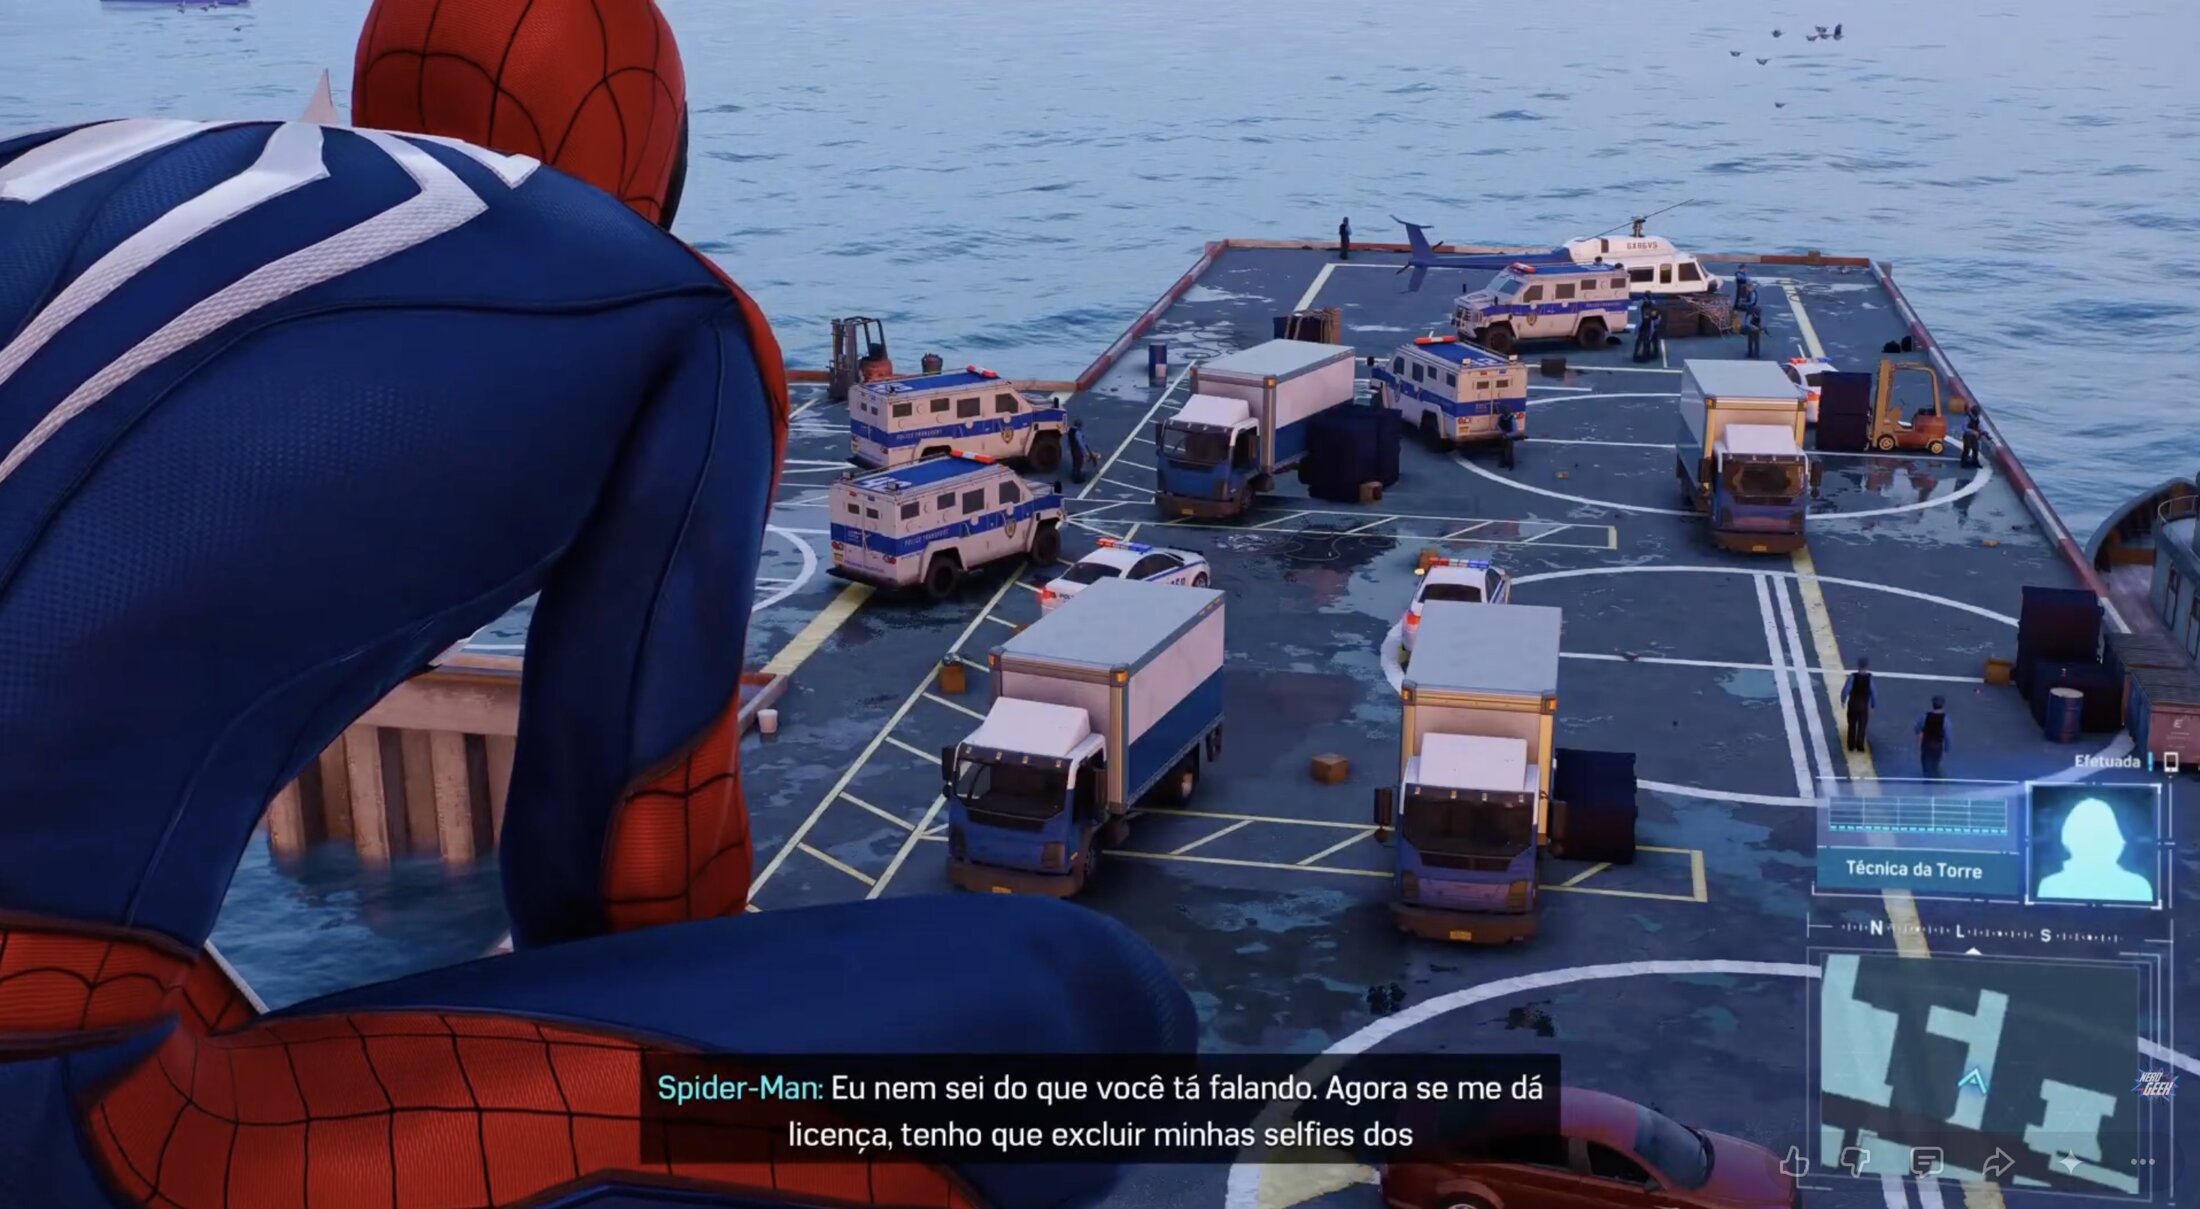
\includegraphics[width=0.9\textwidth]{imagens/spider_man/spider_man.jpg}
    \caption{Captura própria de \textit{Marvel's Spider-Man Remastered}.}
    \label{fig:spider-man}
\end{figure}

\begin{figure}[H]
    \centering
    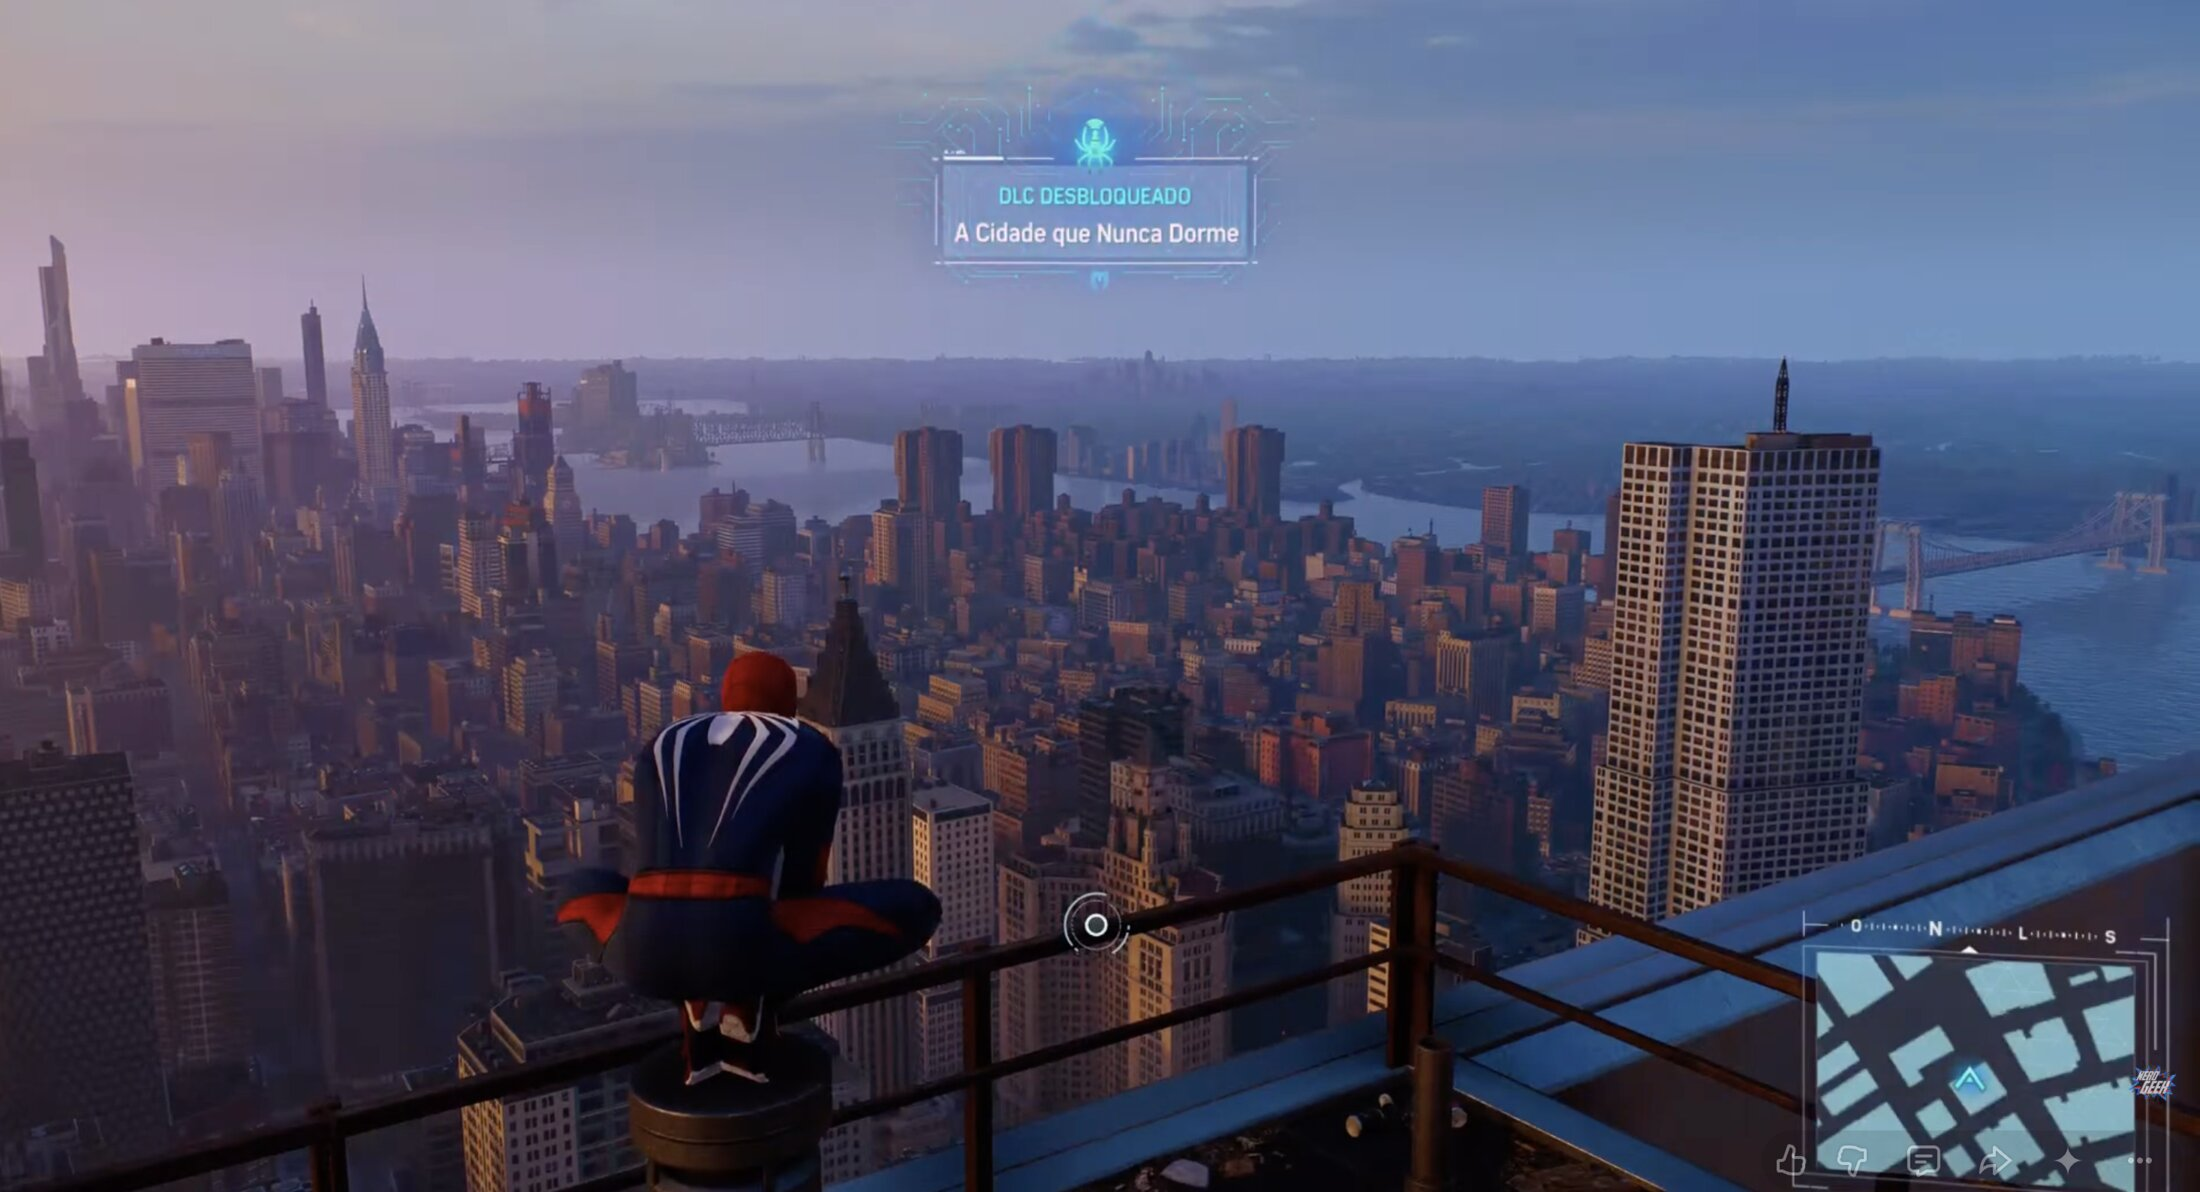
\includegraphics[width=0.9\textwidth]{imagens/spider_man/spider_man02.jpg}
    \caption{Segunda captura própria de \textit{Marvel's Spider-Man Remastered}.}
    \label{fig:spider-man-02}
\end{figure}

\begin{figure}[H]
    \centering
    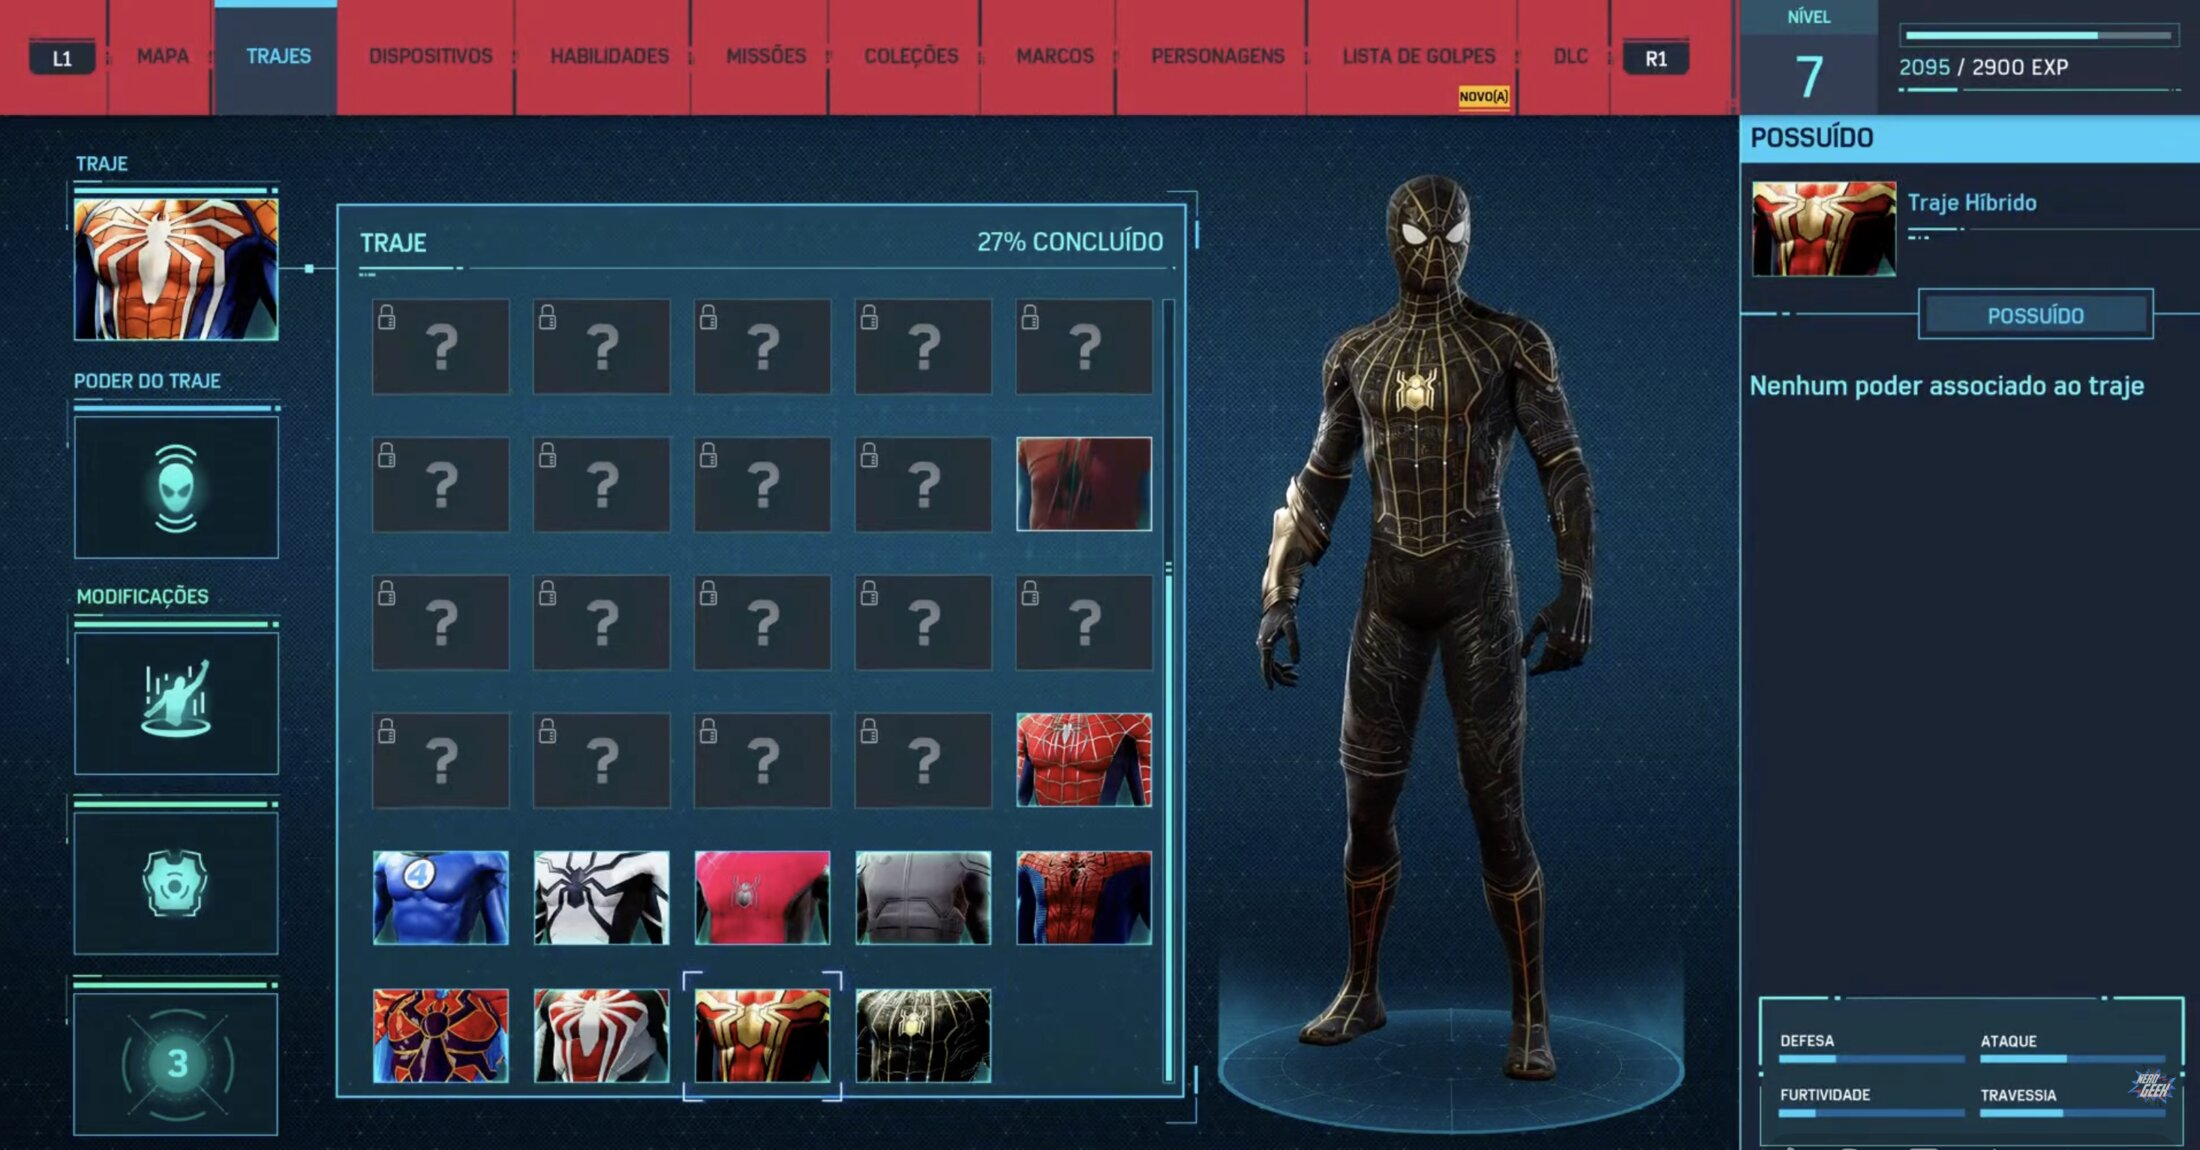
\includegraphics[width=0.9\textwidth]{imagens/spider_man/spider_man03.jpg}
    \caption{Terceira captura própria de \textit{Marvel's Spider-Man Remastered}.}
    \label{fig:spider-man-03}
\end{figure}

As capturas apresentadas nesta seção servem como complemento visual
à análise do jogo. Embora uma imagem estática não permita observar
diretamente os processos internos de aplicação das coordenadas UV,
ela permite analisar o resultado visual das texturas e materiais
durante o gameplay.

\section{Limitação das Capturas}

As capturas de tela permitem analisar o resultado visual apresentado
pelos jogos, porém não revelam diretamente informações internas da
implementação, como os valores das coordenadas UV, os shaders
utilizados ou as funções responsáveis por eventuais efeitos
procedurais.

Por esse motivo, as capturas são complementadas pelas demonstrações
em vídeo apresentadas na seção seguinte. Os vídeos permitem observar
os jogos em execução e diferentes momentos do gameplay, fornecendo
uma evidência complementar às imagens estáticas.